\chapter*{Discussion}
\label{ch:discussion}
The results presented in the previous chapter show general
uncertainty in the models. This has a few possible explanations:
one of the most likely is general overlapping of features. One of the most likely
explanations is the significant overlap of features.\\

There are clear indications of this issue in the performances of neural networks,
particularly the recurrent architecture. This is evident during training, where
significant improvements in training accuracy occur only in later epochs, as shown
in the training and validation accuracy plot (figure[...]):
once training accuracy begins to rise meaningfully, the model quickly overfits.
Additional insights are provided by the confusion matrix and class-wise accuracy
plot (figures [...]), which consistently
show a dominant class with a high number of predictions and a secondary class
with relatively high accuracy, while the remaining classes receive significantly
fewer predictions overall.\\

The convolutional architecture exhibits similar behavior, albeit less prominently
(figures~\ref{fig:cnn_train_val_acc},~\ref{fig:cnn_classacc},~\ref{fig:cnn_confmatr}).
In this case, training accuracy improves earlier in the epochs,
but with minimal corresponding gains in validation accuracy.
The confusion matrix and class-wise accuracy plot reveal analogous patterns, though
to a lesser extent.\\

To address this issue, one solution could be applying a filter to exclude the most
common words, allowing the remaining words to better convey clear emotional
meanings. Another potential unexplored approach is the use of custom
metrics during training that focus on class-wise accuracy instead of overall model
accuracy.\\

% \section*{Explainability analysis}
Another probable issue is the fallacy of the generated ground truth, which may
also contribute to the poor performance and could be linked to the vague distinction
between classes.
This possibility can be investigated through explainability analysis, with an
example provided below (figure~\ref{fig:expl}).

\begin{figure}[H]
    \centering
    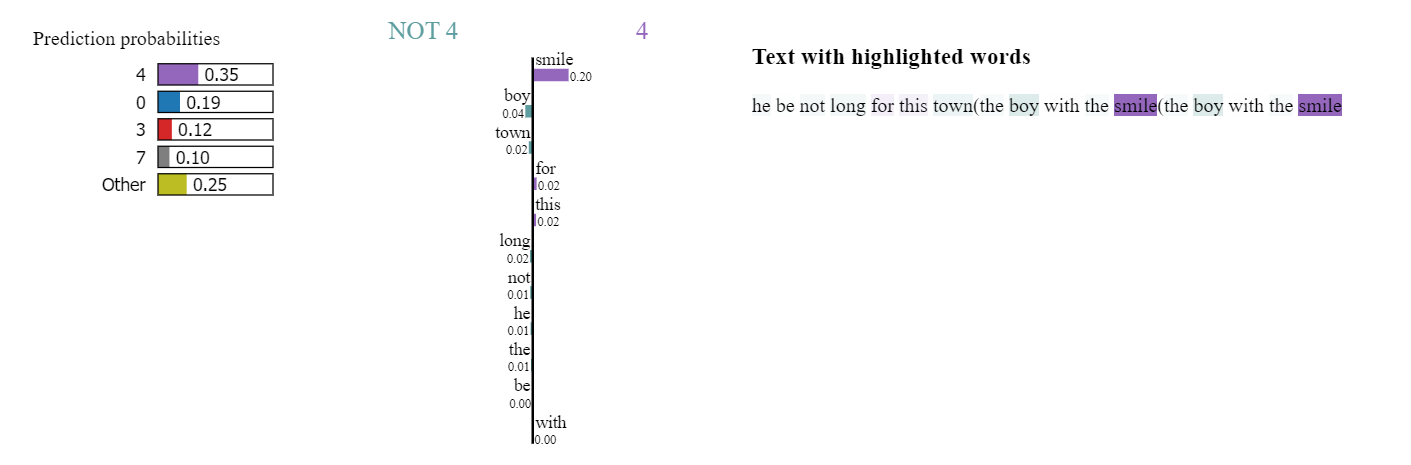
\includegraphics[scale= 0.55]{pictures/expl.png}
    \caption{Explainability - visualization}
    \label{fig:expl}
\end{figure}

The left section of the graph displays the
predicted probabilities for each class. In the center section
feature importances are ranked from most to least relevant and divided into two
groups: on the right
features with a positive influence on the predicted label; on the left, those
with a negative influence that suggest the model should consider other classes.
The right section of the graph highlights the values of the most important
features, using bright colors to indicate features with a positive influence on the
prediction.

The example in question illustrates a prediction where the model assigned the label \textit{joy} to the stanza under analysis, but the expected label, assigned by the ALBERT model, was \textit{sadness}.
However, the word \textit{smile}, which is brighty highlighted, intuitively suggests that \textit{joy} might be a more plausible class for this stanza, even one that ALBERT could reasonably assign. 
This observation raises a critical issue: the transfer learning approach used to create the ground truth appears to have some limitations; in some instances the SVC model assigns a label that seems more contextually appropriate for the stanza, 
yet it differs from the supposedly correct label provided by ALBERT.\\


One possible solution is to switch to a different pseudo-labeling model.
Alternatively, using probability vectors rather than direct classification for
labeling could guide the models toward a regression-based approach. This strategy
may provide more informative inputs for the models and facilitate a deeper
understanding of their performance issues, helping to identify where and why they
struggle.

